In the previous section, the overall structure of the components were looked at. In this part, the model component and function component is going to looked at more thorough, based on previous sections.

\subsubsection{Model Component}

The model component was the part which only had what was called the DB component, in the previous figure. What is included here is actually the original class structure, which is now going to be inserted into the component structure, after it has been updated. This update is based on the event table which was created in the problem area analysis, and with implementation in mind.

Following the theory, the class diagram has been updated to become the model component, taking into consideration private and shared events, and whether or they’re iterative or singular. For example, the add/remove friend events become classes for themselves, and is a part of the class which it had a singular iterative connection with. The other add/remove for the media had a shared iterative connection, so it’s more open how this is going to be showed on the new class diagram. In the Figure \ref{ModelComponent} you can see it as a new layer between the media interested person and the media, and is called the medialist.

\begin{figure}[htb]
\centering
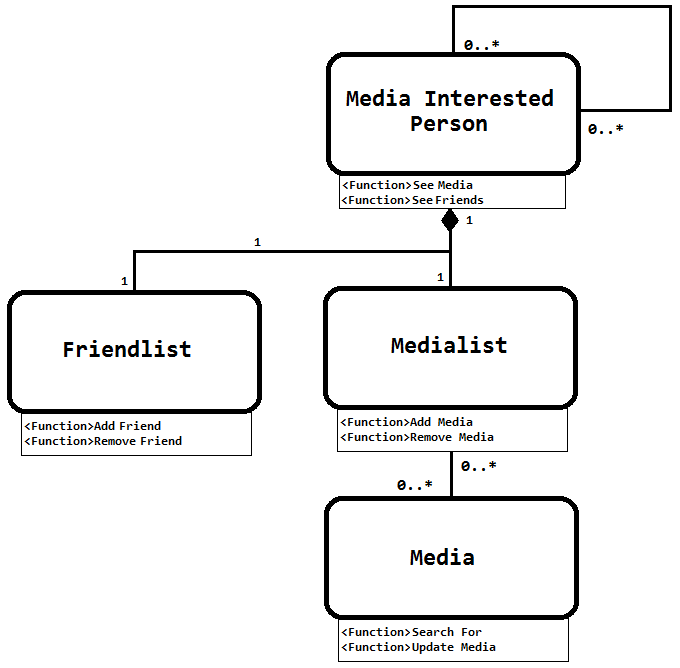
\includegraphics[width=0.7\textwidth]{Images/modelcomponent.png}
\caption{The model component with associated functions}
\label{ModelComponent}
\end{figure}

\subsubsection{Function Component}

The function component is going to be made by going back to the functions which was defined in a previous section, and adding them to the updated component diagram. See Figure \ref{FullComponents}. Their placement is dependent on how many classes have a relations to the specific function. If a function only affects one type of class, then the function can be added directly to the class inside the model komponent. If it affects several, then it should be a separate component inside the function component, pointing the classes in the model component on which it has effect. This can also be seen in Figure \ref{ModelComponent}.

For example, the ‘Generate Recommendations’, works not only on media in the system, but also on users, which it generates media recommendations for. It was already defined in the function component prior to this, this just cements its position there. There is things like add/remove media and friends, which is limited to only one kind of class, and is therefore attached to that class in the model component.

\begin{figure}[htb]
\centering
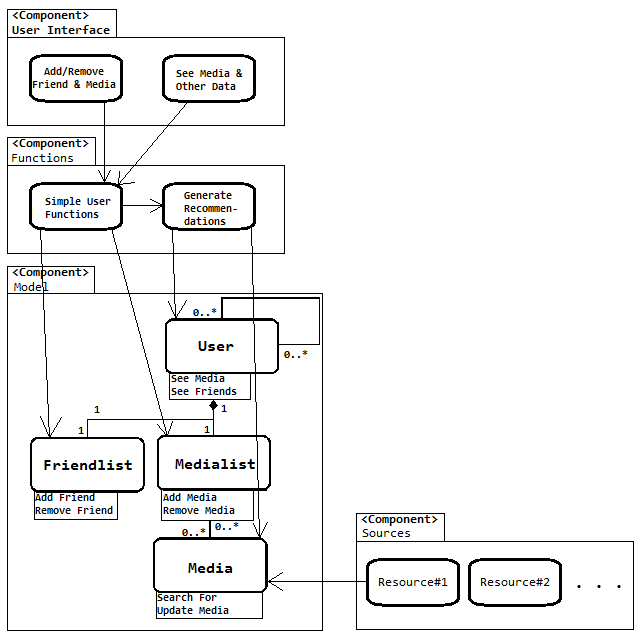
\includegraphics[width=0.6\textwidth]{Images/FullComponents.png}
\caption{The full component structure}
\label{FullComponents}
\end{figure}